\chapter{Conclusiones}
\label{chap:conclusiones}


\drop{C}{omo} conclusión general el resultado del proyecto no solo ha sido bueno, sino que teniendo en cuenta las fuertes restricciones de presupuesto, las limitaciones debido a la falta de información y conocimientos de algunas de las herramientas, ONCOSUP ha sido realmente un éxito. JHipster, a pesar de las complicaciones al inicio del proyecto por el desconocimiento de la herramienta, ha sido de grandísima ayuda, facilitando y agilizando el trabajo de forma excepcional. El inicio del proyecto fue algo lento, por la necesidad de aprender el funcionamiento de JHipster y Angular 5, herramientas con las que ninguno de los integrantes del equipo había trabajado antes; pero las investigaciones acerca de las herramientas, la ayuda entre integrantes del equipo y en ocasiones el ensayo y error, han hecho que JHipster haya dado los resultados esperados, y que el equipo realmente valore este tipo de herramientas que están en auge, mejoran cada día y nos obligan a mantenernos actualizados.

Por otro lado, desde el punto de vista personal de la autora, la experiencia haciendo el FORTE ha sido muy enriquecedora. Le ha permitido aprender nuevas tecnologías y formas de trabajar de las que en la carrera solo había oído hablar, además de adentrarse en el mundo laboral dentro del ambito de la informática. Aprender cómo es el flujo de trabajo dentro de una empresa, en un proyecto real es algo que será muy útil de cara al futuro, ayudándo a los recién graduados a perder ese ``miedo'' que da buscar el primer trabajo y hacer las primeras entrevistas, además de aportar una experiencia extra antes de entrar definitivamente en el mundo laboral.

En cuanto a IECISA, la acogida fue muy buena y la autora se sintió casi desde el principio como una más del equipo, gracias al buen ambiente de trabajo y entre compañeros. No sentirse fuera de lugar animó a la autora a entrar en la dinámica de trabajo fácilmente y querer participar desde el primer momento.

En resumen, la realización de este Trabajo de Fin de Grado con el convenio FORTE le ha parecido a la autora una oportunidad única que ofrece una experiencia totalmente distinta a lo vivido durante el grado que además muy probablemente abrirá puertas al alumno que participe en él.

\section{SCRUM}
\label{sec:conclusionesScrum}

Desde el punto de vista del marco de trabajo seguido en ONCOSUP, SCRUM, el resultado ha sido muy satisfactorio para la autora y todo el equipo implicado en el desarrollo. SCRUM fomenta el trabajo en equipo, la interacción, la comunicación, la proactividad, entre muchas otras características, todas ellas hacen que, si los miembros del equipo participan, el ambiente dentro del proyecto sea muy bueno y los integrantes tengan ganas de trabajar y sacarlo adelante.

Desde el punto de vista de la autora el trabajo con SCRUM ha dado muy buenos resultados. A pesar de que algunos de los riesgos que se planificaron al principio se materializaron, el equipo tuvo un plan de mitigación que se llevó a cabo, asegurándose de haber hecho todo lo que estaba en su mano para evitarlos. En lo referente a los problemas que ha habido a lo largo del desarrollo, es reconfortante saber que alguno son bastante comunes y que en general las soluciones son similares a las que se han dado en ONCOSUP, como se puede leer en el capítulo ``CÓMO HACEMOS RETROSPECTIVAS DE SPRINT'' de \emph{SCRUM y XP desde las trincheras} \cite{scrumXP}, en el que se habla de los problemas más habituales que se detectan en las retrospectivas.

Además el marco de trabajo captó la atención de la autora lo suficiente como para animarse a hacer su propia aportación y realizar un pequeño estudio acerca de la confianza, la visión y distintos puntos de SCRUM, desde el punto de vista de la comunidad de proyecto. Los resultados de este análisis se pueden ver en la sección \ref{sec:valorAñadido}.

\section{JHipster}
\label{sec:conclusionesJhipster}

En cuanto a JHipster, los resultados han sido incluso mejores que los esperados. Se ha conseguido cubrir todo el alcance del proyecto en el tiempo que se había previsto. 

JHipster proporciona una arquitectura con una aplicación lista para usar, que requiere por parte del equipo de desarrollo implementar los cambios necesarios para que cumpla con los requisitos del cliente. Esto permite al equipo centrarse en desarrollar la funcionalidad, ahorrando mucho trabajo. 

Por otro lado si se consulta el número de horas que se han dedicado al proyecto, se obtiene una cifra de unas 1.240 horas, que comparado con las 840 que se estimaron al inicio del proyecto puede parecer mucho, pero la diferencia no es tan grande teniendo en cuenta que: es la primera vez que se trabaja con la herramienta y la estimación se basaba en proyectos similares, pero no iguales; el equipo tuvo que dedicar tiempo a estudiar y aprender; y que en esas horas están también las que registró la autora, con cuya participación no se contaba al inicio del proyecto.

La autora ha querido realizar un pequeño análisis de la herramienta haciendo una comparativa de la aplicación recién generada, y la aplicación tal y como ha quedado tras trabajar en ella. Se ha decidido realizar un conteo de líneas para poder ver cuánto ha crecido la aplicación en su desarrollo. Para realizar este recuento se ha usado la herramienta \emph{Cloc} \cite{cloc}, un proyecto cuyo fin es ayudar a realizar este tipo de análisis, permitiendo saber el total de líneas blancas, comentadas y de código. Permite entre otras opciones además mostrarlas ordenadas por lenguajes, contar solamente archivos con cierta extensión o excluir directorios o archivos según un patrón.

La figura \ref{fig:clocLimpio} muestra un conteo de las líneas que genera JHipster para ONCOSUP, mientras que, la figura \ref{fig:clocLimpio} refleja el recuento de líneas una vez implementada toda la funcionalidad que se entregó al final del proyecto. 

\begin{figure}[!h]
\begin{center}
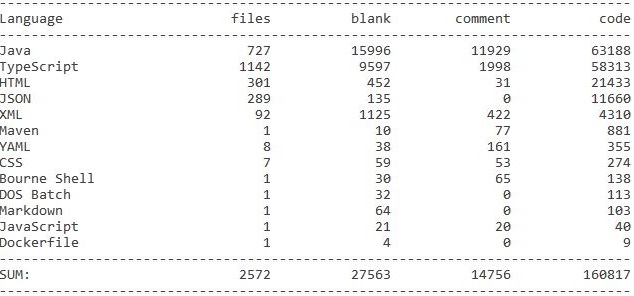
\includegraphics[width=1\textwidth]{clocONCOSUPlimpio}
\caption{Recuento de líneas de código al generar el proyecto}
\label{fig:clocLimpio}
\end{center}
\end{figure}

\begin{figure}[!h]
\begin{center}
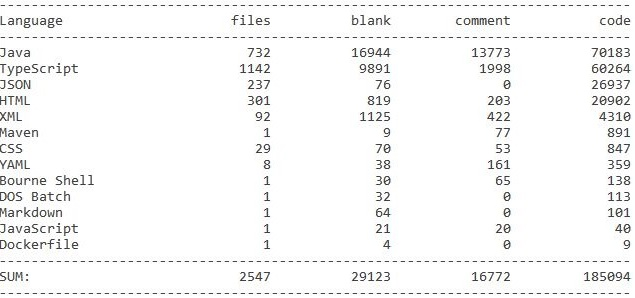
\includegraphics[width=1\textwidth]{clocONCOSUPfinal}
\caption{Recuento de líneas de código al finalizar el proyecto}
\label{fig:clocFinal}
\end{center}
\end{figure}

Analizando los números se puede observar que la mayor cantidad de líneas que ha tenido que añadir el equipo han sido en Java, unas 7.000 líneas, lo que tiene sentido, teniendo en cuenta que ha habido que adaptar el negocio de la aplicación a lo que se necesitaba para ONCOSUP. Se han añadido unas 2.000 líneas en TypeScript, lo cual es razonable ya que los archivos escritos en este lenguaje son los que se encargan del tratamiento de los datos en el cliente. Debido a que ha habido que retocar la maquetación se puede observar un incremento de archivos \emph{css} y, en consecuencia, un aumento de líneas.

Es curioso que en los archivos HTML lo que se ha hecho ha sido reducir el número de líneas, esto se debe a que en la mayoría de casos se han eliminado campos o botones innecesarios, y la nueva maquetación de las pantallas requería menos líneas.

En el cómputo global, la aplicación final tiene un total de 185.094 líneas, 24.277 más que las 160.817 generadas inicialmente. Lo que deja claro que a pesar de que el equipo ha trabajado mucho y ha añadido mucha funcionalidad al equipo, JHipster ha ayudado mucho a que el proyecto salga adelante. Un proyecto de esta magnitud no habría sido posible sin toda la ayuda que JHipster ha dado al equipo.

\section{Objetivos cumplidos}
\label{sec:objetivosCumplidos}

A pesar de lo ajustado que se ha ido de tiempo, finalmente se pudieron completar los cinco objetivos específicos del proyecto, completando así el objetivo general. Estos objetivos son:

\begin{itemize}
	\item Objetivo 1: Estudio Preconsulta. Se comienza a trabajar en este objetivo desde el primer sprint, y a pesar de haberse planeado finalizarlo para la finalización del sprint 2, fue necesario alargar su desarrollo un sprint más, habiendo sido completado al acabar el sprint 3.
	\item Objetivo 2: Consulta de Seguimiento. Cuando el primer objetivo estuvo prácticamente acabado se comenzó a trabajar en el segundo, es decir durante el tercer sprint. La cantidad de elementos que conformaban la consulta resultó en que el equipo tuvo que trabajar en este objetivo hasta el último día del proyecto, habiéndolo acabado durante el sexto sprint.
	\item Objetivo 3: Informes. Una vez la consulta estuvo lo suficientemente avanzada, se inició el trabajo en el objetivo 3. Esto fue en el sprint 5, en el que se trabajó en el filtro, y se finalizó con la impresión en el sprint 6.
	\item Objetivo 4: Administración de Usuarios y Administración de Protocolos. Como se explicó en la sección \ref{sec:ObjetivosEspecíficos}, era necesario comenzar a trabajar en este objetivo para poder cerrar el primero, así que en el primer, segundo y tercer sprint se completó gran parte de las tareas necesarias para cumplir con el objetivo, quedando parado su avance hasta el sexto sprint, donde finalmente se completó.
	\item Objetivo 5: Exportación de datos. Para exportar los datos introducidos en la aplicación era imprescindible saber con certeza que la estructura de los datos no iba a cambiarse. Como se ha trabajado de forma ágil se han tenido que hacer múltiples modificaciones durante el desarrollo, así que este objetivo se decidió abordarlo en el sexto sprint, cuando se sabía con seguridad que no habría más cambios.
\end{itemize}

Además, es importante mencionar que al acabar el sprint 3 ya se había acabado el MVP. El avance y cumplimiento de los objetivos ha sido rápido y organizado, lo que ha permitido completarlos todos y no tener que dejar nada sin abordar.


\section{Objetivos personales}
\label{sec:ObjeticosPersonalesConsulsion}

La autora cree que se han cubierto de sobra sus objetivos personales. Como ya se justificó en el capítulo \ref{chap:objetivos} y con lo redactado en el capítulo \ref{chap:resultados} queda más que claro durante la participación de la autora en ONCOSUP se han tocado diferentes aspectos de esas competencias.

En cuanto a la ampliación de conocimientos, la autora está más que satisfecha. Sus conocimientos respecto a herramientas como JHipster, Angular 5, \emph{JIRA}, \emph{Confluence} o SCRUM, eran mínimos. Aunque está claro que aún hay margen para seguir aprendiendo y ampliando conocimientos, la estancia en IECISA ha sentado una buena base de conocimientos que permiten a la autora desenvolverse con más facilidad, tanto con las herramientas mencionadas, como en el ambiente de trabajo en la empresa.

\section{Un estudio de valor añadido: Valoración de SCRUM}
\label{sec:valorAñadido}


Durante el desarrollo de ONCOSUP la autora tomó la iniciativa de pasar unos breves cuestionarios al final de cada sprint a los participantes del proyecto, con el fin de ver qué tan bien funciona SCRUM y cómo ayuda a cambiar, para bien o para mal, la opinión de los involucrados en el proyecto.

La herramienta utilizada  para la realización y gestión de las encuestas fueron los Formularios de Google \cite{forms}, que permite crear, modificar o incluso duplicar formularios de forma rápida y sencilla. También, muestra un breve análisis de las respuestas, incluyendo la posibilidad de exportar los resultados en una hoja de cálculo, lo que facilitará mucho la recopilación y procesado de los datos.

Se quiso valorar por un lado las sensaciones respecto al proyecto durante su desarrollo y por otra parte se quiso medir en la medida de los posible cómo el equipo considera que está desempeñando en lo referente a los valores de SCRUM. De esta forma, se les pide que respondan a las siguientes preguntas valorando del 1 al 5, siendo 1 muy poco y 5 mucho:

\begin{itemize}
\item Sensaciones respecto al proyecto
	\begin{itemize}
		\item ¿Cuál es tu grado de confianza relativo al éxito del proyecto?
		\item ¿Cuál es tu grado de satisfacción respecto al avance del proyecto en este sprint?
		\item El sentimiento de ``ownership'' (Pertenencia, implicación...) se corresponde con el nivel de entrega e inversión personal en el proyecto y puede variar 			por muchos factores a lo largo del proyecto. ¿Cómo valoras tu sentimiento de ``ownership'' tras este sprint?
	\end{itemize}
	\item Valores de SCRUM
	\begin{itemize}
		\item Compromiso. Estar comprometidos con el equipo y el objetivo del sprint, de tal forma que al acabar el trabajo se comprueba si es posible ayudar al resto 			del equipo a alcanzar el objetivo.
		\item Foco. Mantener los ojos en el objetivo del sprint y no dejarse distraer por preferencias personales o el CEO (\emph{Chief Executive Officer}, el máximo 					responsable) si eso hace peligrar el objetivo del sprint.
		\item Franqueza. Ser transparentes acerca de cómo lo está haciendo el equipo y ser abierto en lo referente a fallos o dificultades que puedan aparecer.
		\item Respeto. Compartir el conocimiento con el equipo y aceptar la profesionalidad del resto de componentes.
		\item Coraje. Ser un profesional que admite errores y se mueve más allá de su propio ego para cambiar la dirección con el fin de resolver problemas complejos.
	\end{itemize}
\end{itemize}




La figura \ref{fig:encuesta1Equipo} muestra los resultados por sprint de las sensaciones del equipo. Se puede apreciar que desde el principio y de forma general las sensaciones eran buenas, comenzando con valores relativamente altos. Hay dos elementos claros en las tres gráficas: todas tienen una tendencia ascendente casi todo el desarrollo, y las tres sufren una caída al final de éste. 

\begin{figure}[!h]
\begin{center}
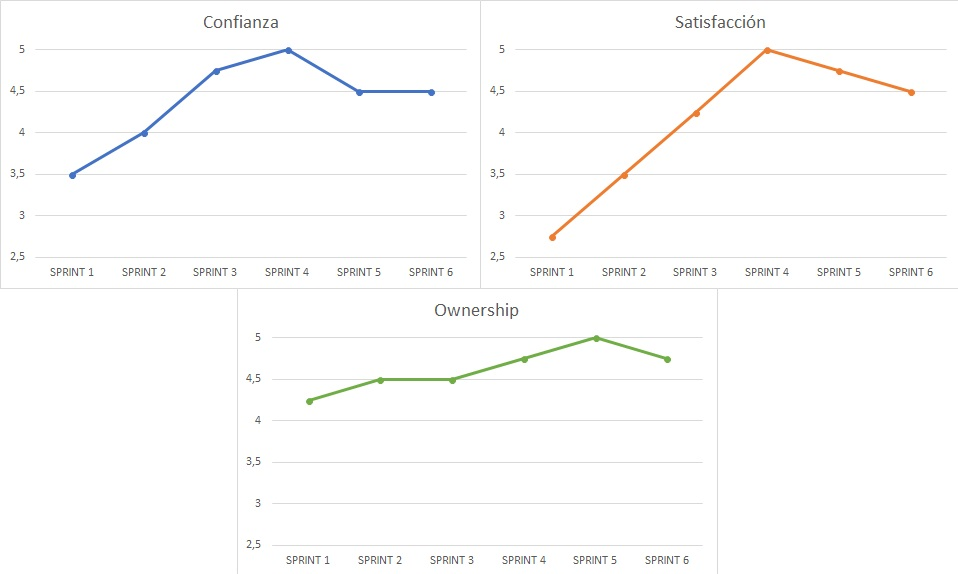
\includegraphics[width=1\textwidth]{encuesta1Equipo}
\caption{Resultados del equipo en la primera parte del cuestionario}
\label{fig:encuesta1Equipo}
\end{center}
\end{figure}

Era de esperar que la valoración de los integrantes del equipo fuese aumentando con el paso de los sprints. Si nos remitimos a lo documentados en el capítulo \ref{chap:resultados}, resulta fácil comprender a qué se debe la bajada hacia el final del proyecto; algunos de los riesgos identificados antes de comenzar con el desarrollo se materializaron, lo que junto a la incertidumbre de si sería posible abarcar todo el alcance del proyecto y la presión de la fecha de finalización cada vez más cerca, probablemente repercutieron en la visión del equipo. 

Cabe mencionar que la caída no es muy drástica, pero lo ideal sería mantener todas las puntuaciones en el 5, el valor más alto. Una mejor gestión de riesgos o un presupuesto menos restrictivo, muy probablemente se habría traducido en puntuaciones más altas hacia el final del proyecto.

Respecto a la valoración del equipo de los valores de SCRUM (fiugra \ref{fig:encuesta2Equipo}), de nuevo se aprecia una esperada tendencia ascendente. En general, todos los números ascienden o se mantienen en valores altos, acabando todos más altos al acabar el proyecto que al empezarlos. La excepción es el compromiso, que tiene una pequeña subida, para al final mantenerse en su valor inicial. Se dio la opción de añadir comentarios referentes a las respuestas en los formularios de los que se puede extraer que quizá la presión o responsabilidades en otros proyectos pudo afectar al compromiso del equipo, explicando que no haya aumentado como el resto de valores.

\begin{figure}[!h]
\begin{center}
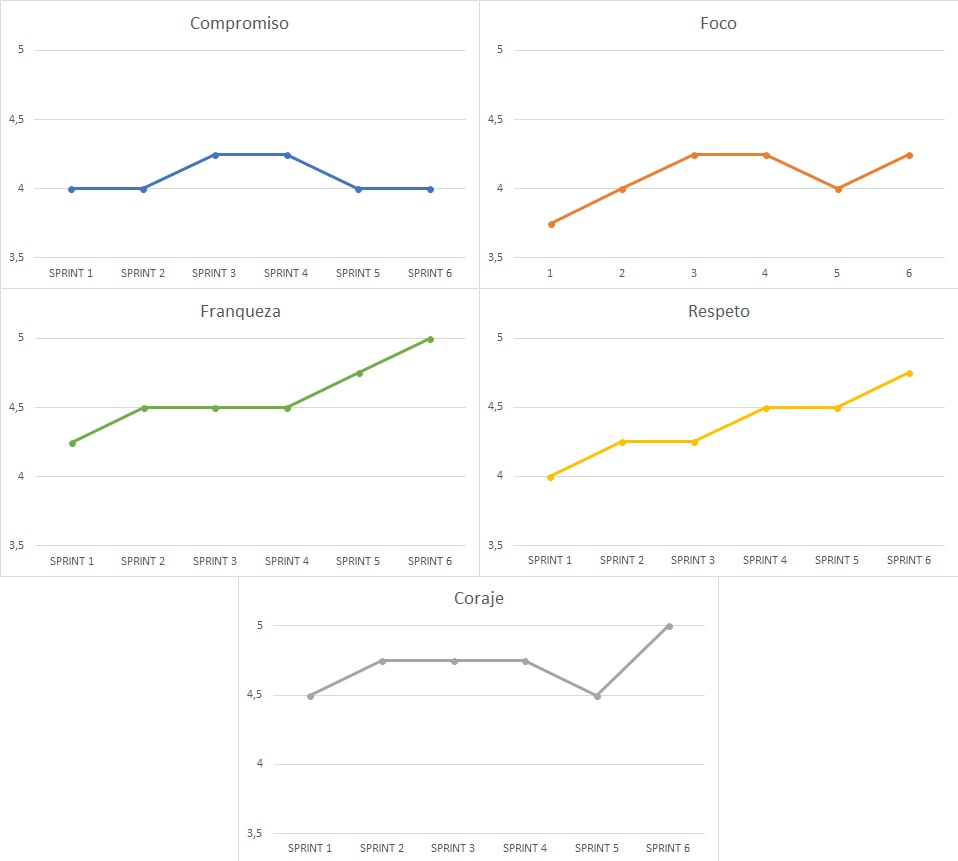
\includegraphics[width=1\textwidth]{encuesta2Equipo}
\caption{Resultados del equipo en la segunda parte del cuestionario}
\label{fig:encuesta2Equipo}
\end{center}
\end{figure}
\clearpage
El balance general es un ascenso, pero se puede apreciar una caída en el coraje y el foco en el sprint 4, que podría ser resultado de la falta de información respecto a los items durante ese sprint. 

Aunque SCRUM se centra en el equipo y lo considera la principal unidad en un proyecto, se considera interesante en este caso analizar las respuestas de la \emph{Product Owner}, ya que no solo era su primer contacto con SCRUM sino que aceptó la responsabilidad sin tener ningún tipo de formación sobre el rol y a sabiendas de que quizá no podría dedicar todo el tiempo necesario.

En la figura \ref{fig:encuesta1Blancaw} se puede ver que las sensaciones son similares a las del equipo, siendo la bajada únicamente en el sexto sprint, lo que puede deberse a que algunos de los riesgos que se dieron durante los últimos sprints no le afectaban directamente mientras que otros en el sexto sprint sí lo hacían, por ejemplo, la instalación fue algo que durante el último sprint hizo peligrar que pudiera acabar usando la aplicación.

\begin{figure}[!h]
\begin{center}
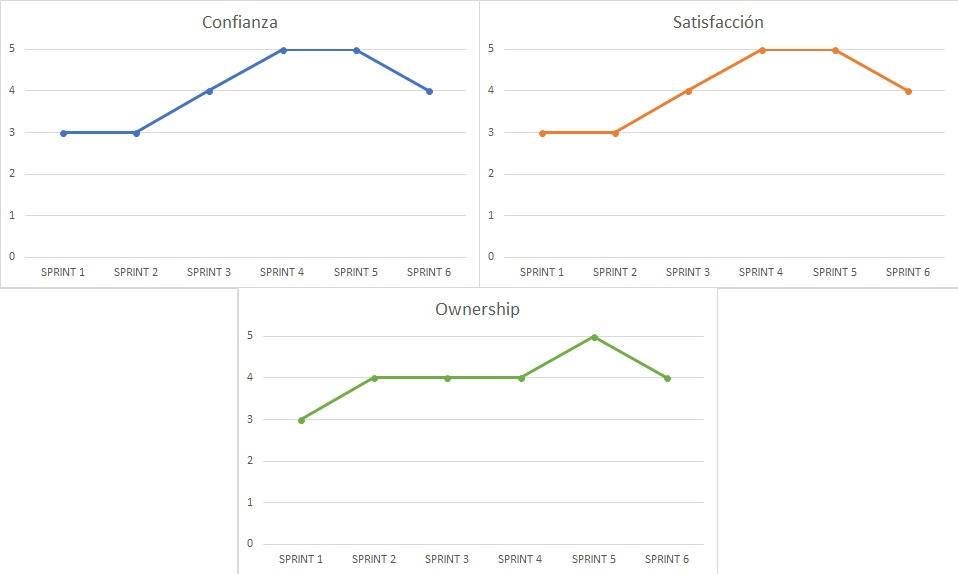
\includegraphics[width=1\textwidth]{encuesta1Blanca}
\caption{Resultados de la Product Owner en la primera parte del cuestionario}
\label{fig:encuesta1Blancaw}
\end{center}
\end{figure}

En cuanto a los valores de SCRUM (figura \ref{fig:encuesta2Blanca}), lo más llamativo es el valor bajo y estable durante todo el proyecto del compromiso, algo de lo que el equipo era consciente, ya que, tal y como se explicó en la sección \ref{sec:inception}, no era posible asegurar que la \emph{Product Owner} tuviera el tiempo necesario que requería el rol. Este es uno de los riesgos de tener un \emph{Product Owner} que no puede dedicarse al completo a su rol. El respeto también ha sido estable durante todos los sprints, pero con valores más altos.
\clearpage
Lo más relevante de estas gráficas es la caída en el sprint 4 del foco, que quizá debido a sus dificultades para estar totalmente comprometida con el proyecto, provocaron que en ese sprint no fuese capaz de proporcionar al equipo toda la información necesaria para completar el trabajo del sprint. Lo realmente interesante, es como esta caída en el foco del \emph{Product Owner} en el sprint 4, se tradujo en una caída general en el foco del equipo en el sprint 5, como se puede ver al comparar con la figura \ref{fig:encuesta2Equipo}.

\begin{figure}[!h]
\begin{center}
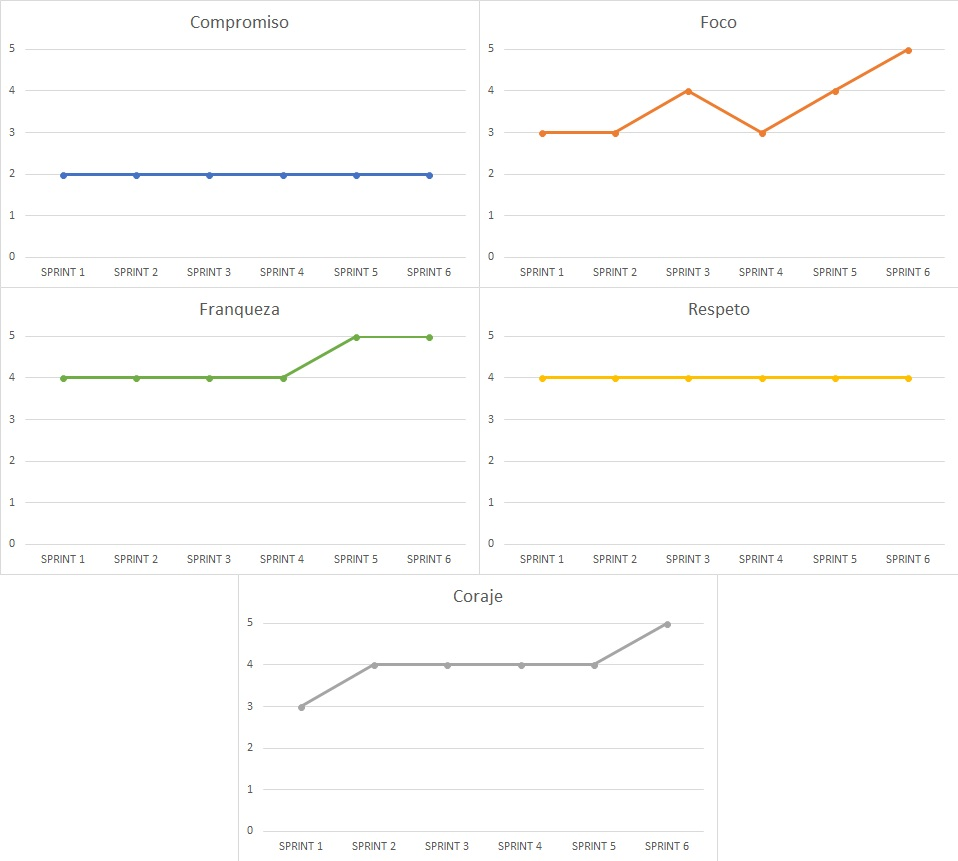
\includegraphics[width=1\textwidth]{encuesta2Blanca}
\caption{Resultados de la Product Owner en la segunda parte del cuestionario}
\label{fig:encuesta2Blanca}
\end{center}
\end{figure}

Finalmente, las gráficas de la figura \ref{fig:SP1vsSP2} son una propuesta sobre cómo mostrar la información recopilada en los cuestionarios de tal forma que permita ver de forma rápida cual ha sido la evolución del equipo desde el inicio hasta el final del proyecto.

\begin{figure}[!h]
\begin{center}
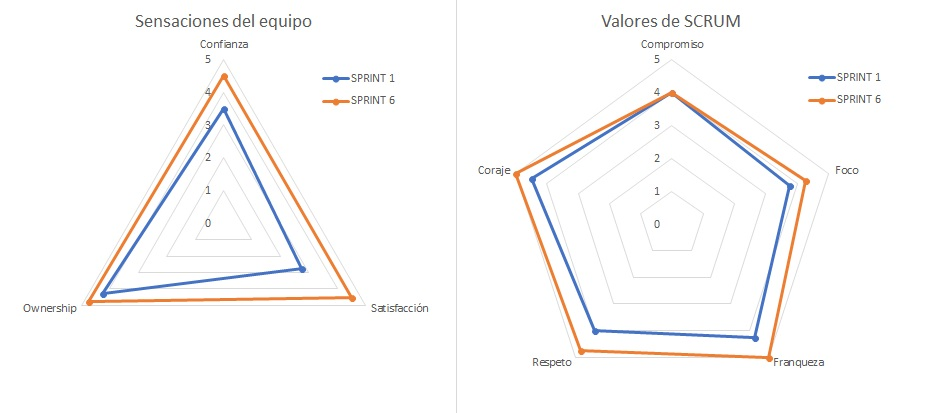
\includegraphics[width=1\textwidth]{SP1vsSP2}
\caption{Comparativa de los resultados del primer y el sexto sprint}
\label{fig:SP1vsSP2}
\end{center}
\end{figure}

En líneas generales, se puede decir que SCRUM es un marco de trabajo que funciona realmente bien. Los resultados en general han sido muy buenos, y las opiniones de los miembros del equipo también. Como opinión personal, la autora considera que la implantación de formularios de este tipo en proyectos de desarrollo, puede ser una herramienta muy buena como soporte para retrospectivas, como herramienta de facilitación para \emph{Scrum Master} para divulgar y promover el cambio cultural a través de la organización poniendo énfasis en este tipo de elementos intangibles y subjetivos que fuera de la agilidad no son fáciles de medir. Podría incluso servir para medir el estado y evolución del equipo de forma similar o complementaria al Modelo de Tuckman \cite{tuckman}.

